
%%%%%%
%
% $Autor: Manoj Selvaraju $
% $Datum: 2024-01-05 11:15:45Z $
% $Pfad: githubtemplate/Template/report/rename.tex $
% $Version: 4620 $
%
%
% !TeX encoding = utf8
% !TeX root = Rename
% !TeX TXS-program:bibliography = txs:///bibtex
%
%%%%%%

\chapter{TensorFlow Lite}

\section{TensorFlow Lite}\label{sec:TensorFlow Lite}

Tensorflow Lite is an optimised environment of TensorFlow models, which is specifically designed for mobile and edge devices, allowing machine learning models to run efficiently on smartphones, embedded systems and other devices with limited computational resources.
Essentially it consists of two components, the model converter, which converts pre-trained TensorFlow models into optimised TensorFlow Lite models and the Interpreter, which enables efficient execution on end devices. \cite{TensorFlowLite:2024} 
%It's primary focus on reducing the size of the existing models and to reduce the latency on low powered devices.

\medskip

TensorFlow Lite has now been officially renamed to LiteRT. Now, LiteRT (formerly TensorFlow Lite) grown beyond its TensorFlow roots to support models from other frameworks like PyTorch, JAX, and Keras. LiteRT continues to serve as the optimized environment for running AI models on mobile devices, embedded systems, and other edge devices, focusing on reducing model size, latency, and energy consumption.
The name change reflects how this high-performance runtime has evolved beyond supporting only TensorFlow models to also include models from other frameworks like PyTorch, JAX, and Keras. LiteRT continues to serve as the optimized environment for running AI models on mobile devices, embedded systems, and other edge devices, focusing on reducing model size, latency, and energy consumption. \cite{Li:2024b}

\section{Why TensorFlow Lite?}
Often the trained models are not to be used on the PC on which they were trained,but on mobile devices such as mobile phones or microcontrollers or other embedded systems. However, limited computing and storage capacities are available there. TensorFlow Lite is a whole framework that allows the conversion of models into a special format and their optimization in terms of size and speed, so that the models can then be run with TensorFlow Lite interpreters on mobile, embedded and IoT devices. \cite{TensorFlowLiteGuide:2024}

However, you cannot train a model directly with TensorFlow Lite, it must first be created with TensorFlow, then you must convert the model from a TensorFlow file to a TensorFlow Lite file using the TensorFlow Lite converter. The reason is that TensorFlow models usually calculate in 32-bit floating point numbers for the neural networks. The weights can assume very small values close to zero. Therefore, the models cannot be run on systems that cannot calculate with long floating point numbers, but only with 8-bit integers. This is especially the case with small AI processors, on which only a few transistors can be accommodated due to size and power consumption. Therefore, the neural network must undergo a transformation, in which long floating-point numbers with varying precision over the representable range of values– floating-point numbers represent the range of numbers around the zero point much more finely than very large or small values– become short integers with constant precision in a limited range of values. \cite{CoralAI:2024}


\section{Working Procedure of TensorFlow Lite}

TensorFlow Lite workflow consists of four steps as illustrated in the figure ~\ref{TensorLiteWorkflow} Here’s how TensorFlow Lite works:  \cite{TensorFlowLite:2024}

\begin{enumerate}
	\item Model Creation
	\item Model Conversion
	\item Model Deployment
	\item Model Optimization
\end{enumerate}

\begin{figure}[h]
	\centering
	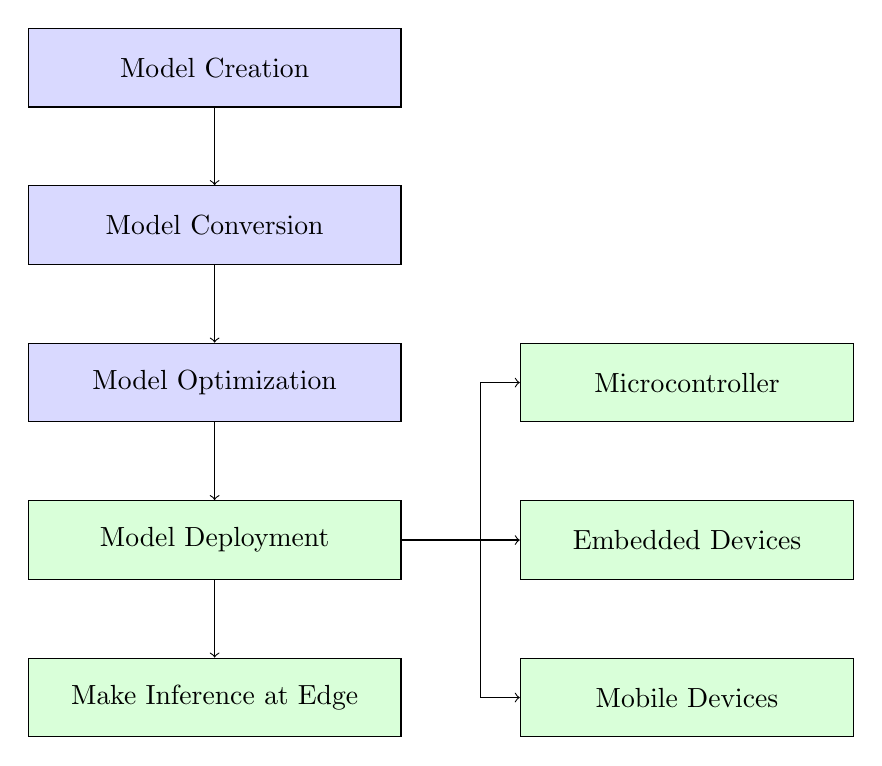
\begin{tikzpicture}[node distance=2cm, auto]
		% Node style
		\tikzstyle{block} = [rectangle, draw=black, fill=blue!15, text width=4.5cm, text centered, minimum height=1cm]
		
		% Nodes
		\node[block] (creation) {Model Creation};
		\node[block, below of=creation] (conversion) {Model Conversion};
		\node[block, below of=conversion] (optimization) {Model Optimization};
		\node[block, draw=black, fill=green!15, below of=optimization] (deployment) {Model Deployment};
		\node[block, draw=black, fill=green!15, below of=deployment] (inference) {Make Inference at Edge};
		
		\node[block, draw=black, fill=green!15, right of=deployment, xshift=4cm, yshift=2cm, text width=4cm] (microcontroller) {Microcontroller};
		\node[block, draw=black, fill=green!15, right of=deployment, xshift=4cm, text width=4cm] (embedded) {Embedded Devices};
		\node[block, draw=black, fill=green!15, right of=deployment, xshift=4cm, yshift=-2cm, text width=4cm] (mobile) {Mobile Devices};
		
		% Arrows
		\draw[->] (creation) -- (conversion);
		\draw[->] (conversion) -- (optimization);
		\draw[->] (optimization) -- (deployment);
		\draw[->] (deployment) -- (inference);
		\draw[->] (deployment.east) -- ++(1,0) |- (microcontroller.west);
		\draw[->] (deployment.east) -- (embedded.west);
		\draw[->] (deployment.east) -- ++(1,0) |- (mobile.west);
	\end{tikzpicture}
	\caption{TensorLite Workflow}
	\label{TensorLiteWorkflow}
\end{figure}


\subsection{Model Creation and Training}
The first step involves creating and training a machine learning model using TensorFlow. 
\\TensorFlow Lite uses TensorFlow models converted into a smaller, more efficient machine learning (ML) model format. You can use pre-trained models with TensorFlow Lite, modify existing models, or build your own TensorFlow models and then convert them to TensorFlow Lite format. TensorFlow Lite models can perform almost any task a regular TensorFlow model can do: object detection, natural language processing, pattern recognition, and more using a wide range of input data including images, video, audio, and text. \cite{TensorFlowLite:2024}

The listing ~\ref{lst:modelCreationTraining} explains the workflow of creating and training a simple neural network model using TensorFlow's Keras API. Also it simplifies a simple example of image classification involving steps in preparing data from MNIST dataset, building, training, evaluating the model for further conversion to TensorFlow Lite format. \cite{TensorFlowLiteExample:2024}

\begin{code}
\begin{lstlisting}[language=Python, caption={Model Creation and Training Example Using TensorFlow}, label={lst:modelCreationTraining}]
	import tensorflow as tf
	from tensorflow.keras.models import Sequential
	from tensorflow.keras.layers import Dense, Flatten
	from tensorflow.keras.optimizers import Adam
	
	# Load the MNIST dataset
	mnist = tf.keras.datasets.mnist
	(x_train, y_train), (x_test, y_test) = mnist.load_data()
	
	# Normalize the images to the range [0, 1]
	x_train, x_test = x_train / 255.0, x_test / 255.0
	
	# Define a simple Sequential model
	model = Sequential([
	Flatten(input_shape=(28, 28)),  # Flatten the 28x28 images into a 1D array of 784 elements
	Dense(128, activation='relu'),  # Hidden layer with 128 neurons and ReLU activation
	Dense(10, activation='softmax') # Output layer with 10 neurons for classification
	])
	
	# Compile the model with an optimizer, loss function, and metric
	model.compile(optimizer=Adam(),
	loss='sparse_categorical_crossentropy',
	metrics=['accuracy'])
	
	# Train the model on the training data
	model.fit(x_train, y_train, epochs=5, validation_data=(x_test, y_test))
	
	# Evaluate the model on the test data
	test_loss, test_acc = model.evaluate(x_test, y_test, verbose=2)
	print(f'\nTest accuracy: {test_acc:.4f}')
	
	# Save the trained model as a SavedModel format (for future conversion to TFLite)
	model.save('saved_model/my_mnist_model')
\end{lstlisting}
\end{code}

\subsection{Model Conversion}
\label{subsec:model_conversion}
Once the model is trained, it needs to be converted into a TensorFlow Lite model. The TensorFlow Lite converter takes a TensorFlow model and generates a TensorFlow Lite model, an optimized FlatBuffer format identified by the file extension \FILE{.tflite}. \cite{TensorFlowLiteModelConversion:2024}

The model conversion can be done using the Python API or the Command
line tool
\begin{itemize}
	\item Command-line Tool: \SHELL{tflite convert}, this allows you to integrate the conversion into your development pipeline, apply optimizations, add metadata and many other tasks that simplify the conversion process.
	\item Python API: \SHELL{tf.lite.TFLiteConverter}, this only supports basic model conversion.
\end{itemize}

The process involves following steps:
\begin{itemize}
	\item \textbf{Select the Model}: The converter accepts the following input model formats.
	\begin{itemize}
		\item \FILE{SavedModel}: A TensorFlow model saved as a set of files on disk.
		\SHELL{tf.lite.TFLiteConverter.from\_saved\_model(model)}
		\item \FILE{Keras model}: A model created using the high level Keras API.
		\SHELL{tf.lite.TFLiteConverter.from\_keras\_model(model)}
		\item \FILE{Keras H5 format}: A light-weight alternative to SavedModel format supported by Keras API.
		\SHELL{tf.lite.TFLiteConverter.from\_keras\_model(model\_loaded\_from\_model.h5)}
		\item \FILE{Models built from concrete functions}: A model created using the low level TensorFlow API.
		\SHELL{tf.lite.TFLiteConverter.from\_concrete\_functions([func], model)}
	\end{itemize}
	The listing ~\ref{lst:modelConversionCode} provides the APIs for the above mentioned models. \cite{TensorFlowLiteInference:2024}
	
\begin{code}
	% Include a specific range of lines from the Python file for Model Conversion
	\lstinputlisting[
	language=Python, 
	firstline=1, 
	lastline=22, 
	caption={Python Code for Converting Models to .tflite}, 
	label={lst:modelConversionCode}
	]{../../Code/TensorFlowLite/ModelConversionCode.py}
\end{code}
	
	\item \textbf{Optimize the Model}: During conversion, various optimization techniques can be applied to make the model more efficient. These includes quantization, Pruning, Clustering.
\end{itemize}

The goal of these optimizations is to make the model smaller and faster while maintaining accuracy.

\subsection{Model Deployment}
After converting the model to a file \FILE{.tflite}, it can be deployed on a variety of devices including mobile phones, embedded systems, and microcontrollers. TensorFlow Lite supports deployment on both Android and iOS platforms, as well as other systems like Arduino.

\subsection{Running Inference}
The term inference refers to the process of executing a TensorFlow Lite model on-device in order to make predictions based on input data. To perform an inference with a TensorFlow Lite model, you must run it through an interpreter. The TensorFlow Lite interpreter is designed to be lean and fast. The interpreter uses a static graph ordering and a custom (less-dynamic) memory allocator to ensure minimal load, initialization, and execution latency. \cite{TensorFlowLiteInference:2024} \cite{GoogleAIEdge:2024}

Here’s the typical process:

\begin{itemize}
	\item \textbf{Load the Model}: The TensorFlow Lite model file \FILE{.tflite} is loaded into the memory, which contains the model's execution graph. 
	The listing \ref{lst:modelLoading} provides the code for Loading and Validating a TensorFlow Lite Model for Microcontroller.

	\begin{code}
	% Include a Model loading line code from the C++ file
	\lstinputlisting[language=C++, firstline=1, lastline=17, label={lst:modelLoading}, caption={Loading and Validating a TensorFlow Lite Model for Microcontroller}]{../../Code/TensorFlowLite/InferenceLoadingModel.cpp}
	\end{code}
	
	\item \textbf{Allocate Tensors}: Build an Interpreter based on an existing model, that is allocating memory for the input and output tensors. 
	The listing \ref{lst:AllocateTensor} provides the reference code for Allocating Tensors for TensorFlow Lite Model Execution on Microcontroller.

	\begin{code}
	%  
	\lstinputlisting[language=C++, firstline=1, lastline=17, label={lst:AllocateTensor}, caption={Allocating Tensors for TensorFlow Lite Model Execution}]{../../Code/TensorFlowLite/InferenceAllocateTensor.cpp}
	\end{code}

	\item \textbf{Set Input Data}: Set input tensor values (Optionally resize input tensors if the predefined sizes are not desired) and fed into the model. 
	The listing \ref{lst:InputData} gives the reference code for setting Input Data for TensorFlow Lite Inference on a Microcontroller.
	\begin{code}
		%  
		\lstinputlisting[language=C++, firstline=1, lastline=17, label={lst:InputData}, caption={Setting Input Data for TensorFlow Lite Inference}]{../../Code/TensorFlowLite/InferenceInputData.cpp}
	\end{code}
	
	\item \textbf{Invoke the Interpreter}: The interpreter runs the model with the input data to produce the output. 
	The listing \ref{lst:InvokeInterpreter} gives the reference code for invoking TensorFlow Lite Interpreter to perform Inference on a Microcontroller.
	\begin{code}
		% 
		\lstinputlisting[language=C++, firstline=1, lastline=17, label={lst:InvokeInterpreter}, caption={Invoking TensorFlow Lite Interpreter to perform Inference on a Microcontroller}]{../../Code/TensorFlowLite/InferenceRunning.cpp}
	\end{code}
	
	\item \textbf{Get Output Data}: The output data is extracted and post-processed to get the final predictions. 
	The listing \ref{lst:OutputData} gives the reference code Extracting and Processing Output Data from a TensorFlow Lite Model																																 on a Microcontroller
	\begin{code}
		% 
		\lstinputlisting[language=C++, firstline=1, lastline=5, label={lst:OutputData}, caption={Extracting and Processing Output Data from a TensorFlow Lite Model}]{../../Code/TensorFlowLite/InferenceOutputData.cpp}
	\end{code}
	
\end{itemize}

% Include a specific range of lines from the Python file for InterfaceCode
%\lstinputlisting[language=Python, firstline=1, %lastline=17]{../../Code/TensorFlowLite/InterfaceCode.py}

\subsubsection{Tensors in TensorFlow Lite}
In TensorFlow Lite, a tensor is a multi-dimensional array that represents the basic data structure used by the library. Just like a vector is a one-dimensional array and a matrix is a two-dimensional array, a tensor can be n-dimensional. Tensors can have different shapes and data types, and they are used for both input and output of the model. \cite{TensorFlowLiteInference:2024}
%\begin{comment}
%Here's a brief overview of tensors
%
%\subsection{Shape} 
%The shape of a tensor defines the number of elements in each dimension. For example, a tensor with shape [2, 3, 4] has 2 elements in the first dimension, 3 elements in the second dimension, and 4 elements in the third dimension.
%
%\subsection{Data Type}
%Tensors can contain different types of data, such as integers, floating-point numbers, or strings. The data type is specified when the tensor is created.
%
%\subsection{Usage in TensorFlow Lite}
%\begin{itemize}
%	\item \textbf{Input Tensors}: These are used to feed the input data into the model. The input tensor shape and data type must match what the model expects.
%	\item \textbf{Output Tensors}: These store the results produced by the model after running inference. The output tensor shape and data type depend on the model's architecture and the specific task it performs.
%\end{itemize}
%
%\subsection{Tensor Examples}
%\begin{itemize}
%	\item If a model expects an input image of size 224x224 with 3 color channels (RGB), the input tensor shape might be [1, 224, 224, 3], where 1 represents the batch size. After running inference, the output might be a tensor of shape [1, 1000] if the model outputs probabilities for 1000 different classes.
%	\item If an object detection model processes an input image of size 300x300 with 3 color channels (RGB), the input tensor shape might be [1, 300, 300, 3]. The output tensor might include bounding boxes, with a shape of [1, 10, 4] where 10 represents the number of detected objects and 4 represents the coordinates of each bounding box.
%\end{itemize}
%\end{comment}




